
%%%% END ARROWS %%%%%%%%%%%%%%%%%%%%%%%%%

%%%%%%%%%%%%%% TIKZ %%%%%%%%%%%%%%%%
\tikzstyle{background rectangle}= [rounded corners, fill=yellow!20, draw=black, rounded corners=1ex]
\tikzstyle{every picture}=[show background rectangle, ->,>=latex,auto,node distance=1.3cm,thick,initial text=,initial where=above,scale=0.8,transform shape]
\tikzstyle{every state}=[draw=yellow!20,line width=4pt,fill=black,minimum size=5pt]

\tikzstyle{loop right}=[in=-30,out=30,looseness=8]
\tikzstyle{loop left}=[in=150,out=210,looseness=8]
\tikzstyle{loop above}=[in=60,out=120,looseness=8]
\tikzstyle{loop below}=[in=240,out=300,looseness=8]

\tikzstyle{loop above right}=[in=5,out=65,looseness=8]
\tikzstyle{loop above left}=[in=105,out=165,looseness=8]
\tikzstyle{loop slightly above left}=[in=125,out=185,looseness=8]
\tikzstyle{loop slightly above right}=[in=5,out=65,looseness=8]
\tikzstyle{loop below left}=[in=195,out=255,looseness=8]
\tikzstyle{loop below right}=[in=285,out=-15,looseness=8]
\tikzstyle{loop slightly below left}=[in=155,out=215,looseness=8]
\tikzstyle{loop slightly below right}=[in=305,out=5,looseness=8]

\tikzstyle{nodeSmall} = [state, node distance=1.5cm, draw=yellow!20, fill=black]
\tikzstyle{finalNode} = [node distance=1.5cm]
\tikzstyle{onEdge}=[fill=yellow!20, pos=0.5]
%%%%%%%%%%%%%% END TIKZ %%%%%%%%%%%%%

\begin{tikzpicture}
\node (GROOVE) {
  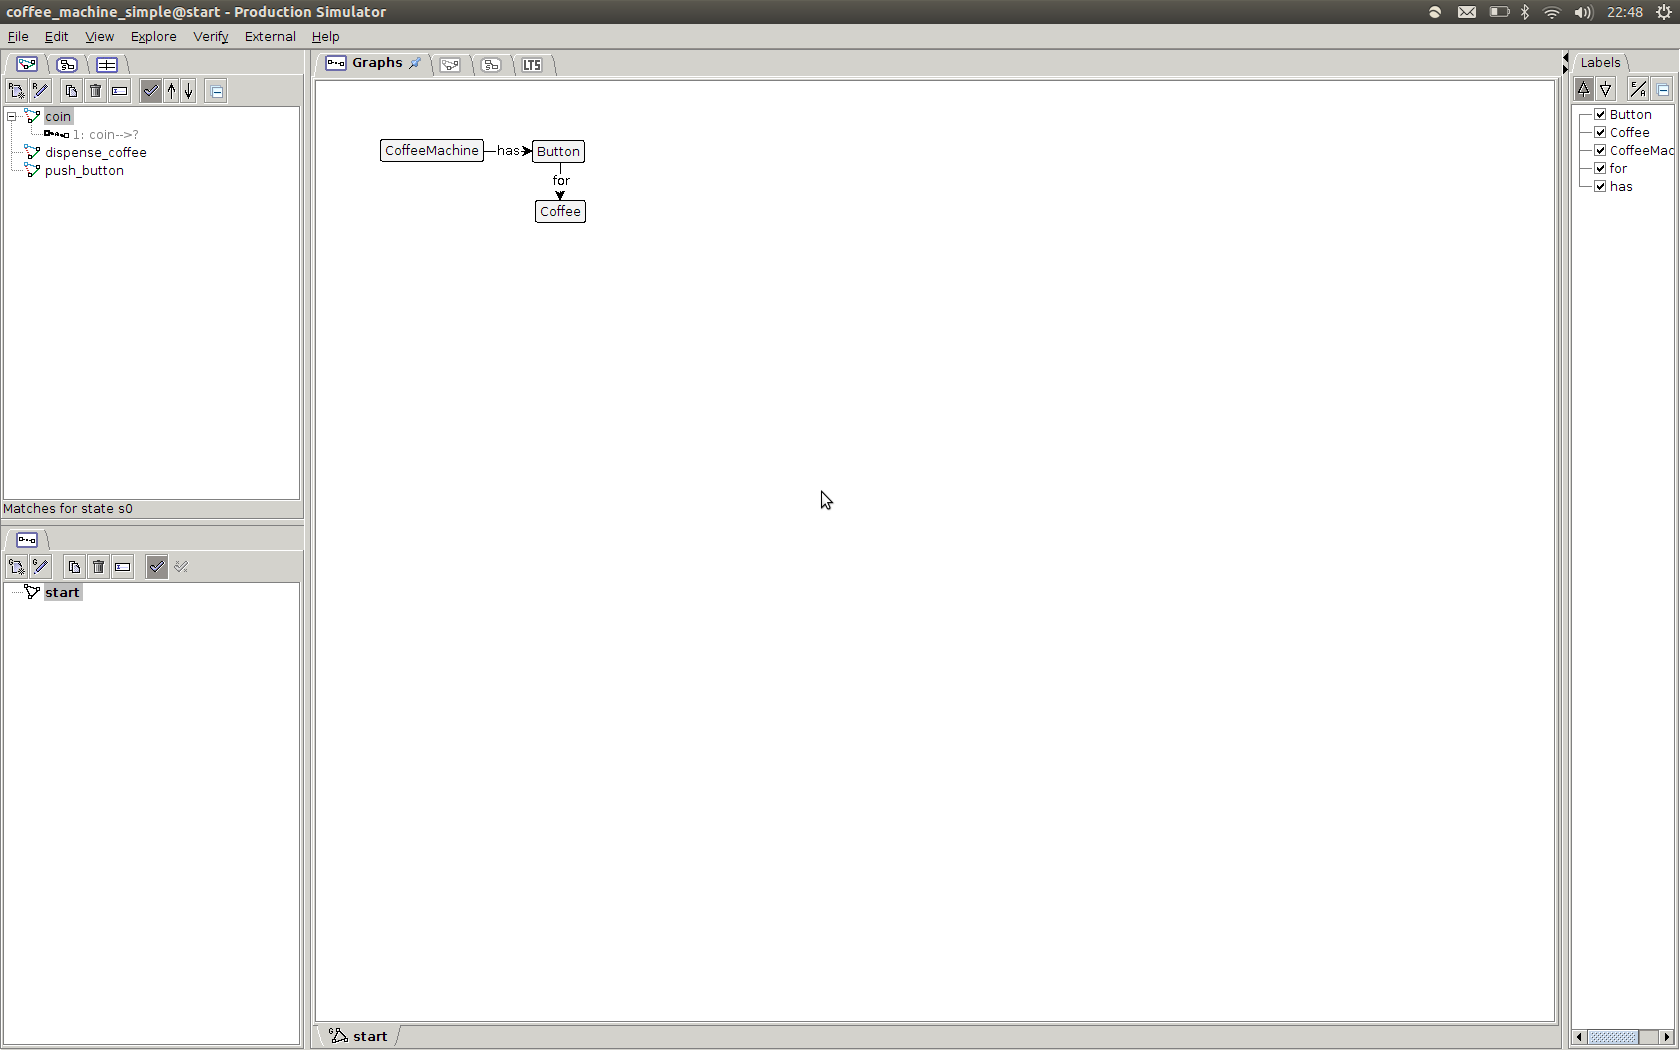
\includegraphics[scale=0.08]{./figures/groove.png}
};
\node (GROOVE TAG) [below=1pt of GROOVE]{\textbf{GROOVE}};
\node (GG2STS) [shape = rectangle, fill = black!30!white, below right=-5pt and -5pt of GROOVE]{\textbf{GG -> STS}};
\node (Cloud) [above right=3cm and 1cm of GROOVE] {
  
\includegraphics[]{./figures/cloud.png}
};
\node (ATM) [right=5cm of GROOVE] {
  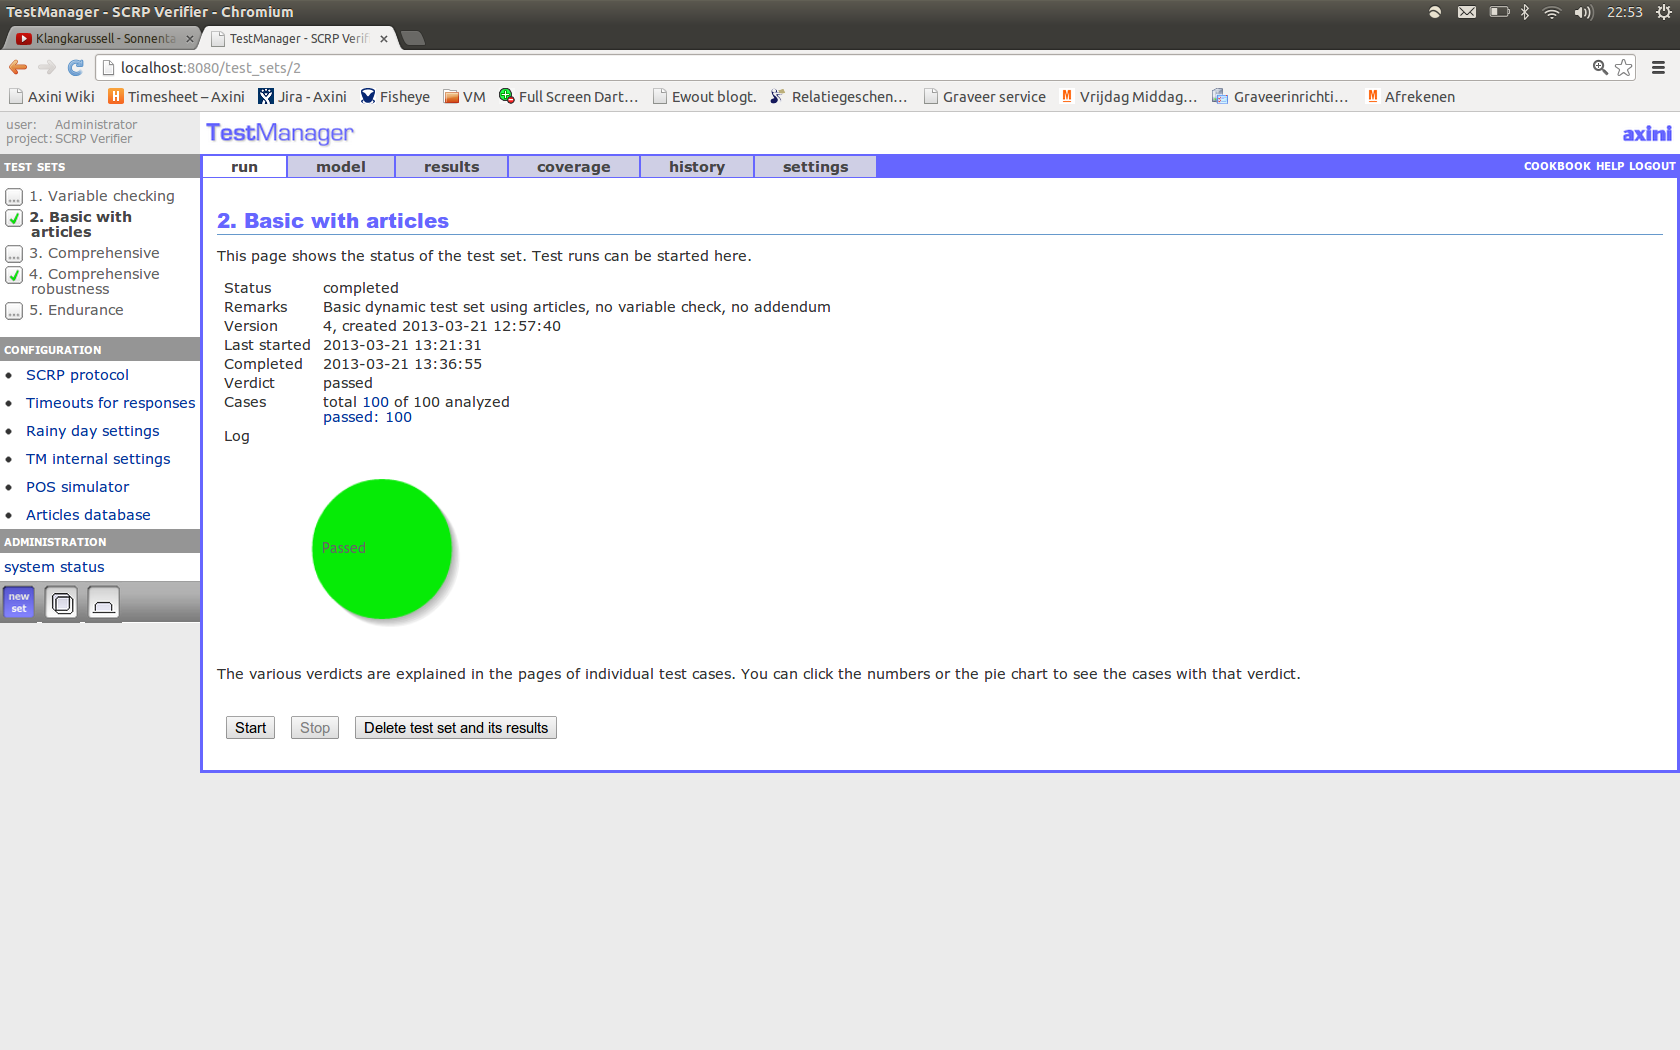
\includegraphics[scale=0.08]{./figures/atm.png}
};
\node (ATM TAG) [below=1pt of ATM]{\textbf{ATM}};

\node (SUT) [above=1.5cm of ATM] {
  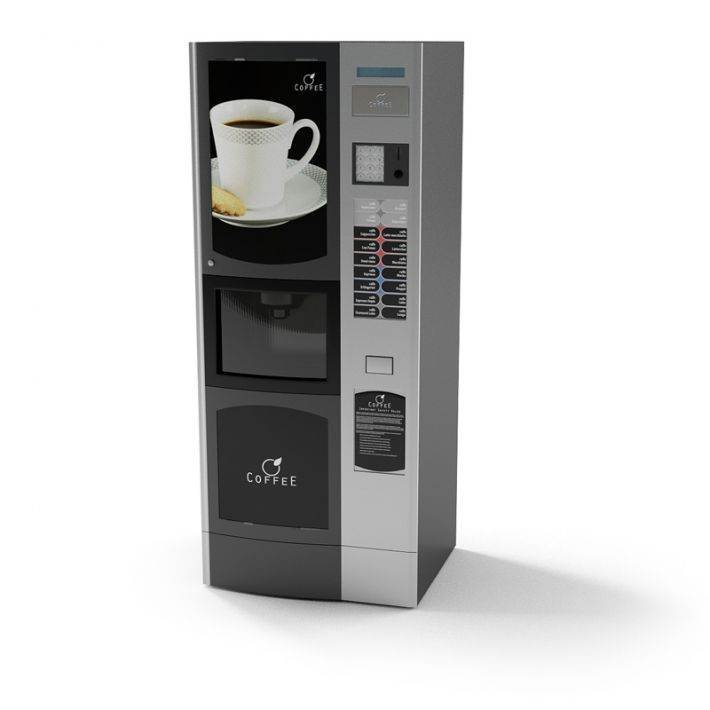
\includegraphics[scale=0.10]{./figures/coffee_machine.jpg}
};

\path ([xshift=2ex]ATM.north) edge node [sloped,midway,above] {input} ([xshift=2ex]SUT.south) ;
\path ([xshift=-2ex]SUT.south) edge node [sloped,midway,above] {output}  ([xshift=-2ex]ATM.north) ;

\path (GROOVE) edge node [sloped,midway,above] {STS}(Cloud) ;
\path (Cloud) edge node [sloped,midway,above] {STS} (ATM) ;
\end{tikzpicture}